\let\negmedspace\undefined
\let\negthickspace\undefined
\documentclass[journal]{IEEEtran}
\usepackage[a4paper, margin=10mm, onecolumn]{geometry}
%\usepackage{lmodern} % Ensure lmodern is loaded for pdflatex
\usepackage{tfrupee} % Include tfrupee package

\setlength{\headheight}{1cm} % Set the height of the header box
\setlength{\headsep}{0mm}  % Set the distance between the header box and the top of the text

\usepackage{gvv-book}
\usepackage{gvv}
\usepackage{cite}
\usepackage{amsmath,amssymb,amsfonts,amsthm}
\usepackage{algorithmic}
\usepackage{graphicx}
\usepackage{float}
\usepackage{textcomp}
\usepackage{xcolor}
\usepackage{txfonts}
\usepackage{listings}
\usepackage{enumitem}
\usepackage{mathtools}
\usepackage{gensymb}
\usepackage{comment}
\usepackage[breaklinks=true]{hyperref}
\usepackage{tkz-euclide} 
\usepackage{listings}
% \usepackage{gvv}                                        
\def\inputGnumericTable{}                                 
\usepackage[latin1]{inputenc}                                
\usepackage{color}                                            
\usepackage{array}                                            
\usepackage{longtable}                                       
\usepackage{calc}                                             
\usepackage{multirow}                                         
\usepackage{hhline}                                           
\usepackage{ifthen}                                           
\usepackage{lscape}
\usepackage{tikz}
\usetikzlibrary{patterns}
\usepackage{multicol}
\begin{document}

\bibliographystyle{IEEEtran}
\vspace{3cm}

\title{GATE-02}
\author{ee25btech11063-vejith}


\maketitle
% \maketitle
% \newpage
% \bigskip
{\let\newpage\relax\maketitle}

\renewcommand{\thefigure}{\theenumi}
\renewcommand{\thetable}{\theenumi}
\setlength{\intextsep}{10pt} % Space between text and floats

\begin{enumerate}[start=1]
\item Choose the most appropriate word from the options given  below to complete the following sentence.\\

A person suffering from  Alzheimer's disease \makebox[2cm]{\hrulefill} short-term  memory loss .

\hfill{(GATE GG 2014)}
\begin{enumerate}
    \item  experienced
\item  has experienced
\item  is experiencing
\item  experiences
\end{enumerate}
\vspace{0.5cm}
\item Choose the most appropriate word from the options given below to complete the following sentence.\\

\makebox[2cm]{\hrulefill}is the key to their happiness; they are satisfied with what they have.

\hfill{(GATE GG 2014)}
\begin{multicols}{4}
    \begin{enumerate}
    \item  Contentment
\item  Ambition
\item  Perseverance
\item  Hunger
\end{enumerate}
\end{multicols}

\vspace{0.5cm}
\item Which of the following options is the closest in meaning to the sentence below?\\

"As a woman, I have no country."

\hfill{(GATE GG 2014)}
\begin{enumerate}
    \item  Women have no country.
\item  Women are not citizens of any country.
\item  Women's solidarity knows no national boundaries.
\item  Women of all countries have equal legal rights.
\end{enumerate}
\vspace{0.5cm}
\item In any given year, the probability of an earthquake greater  than Magnitude $6$ occurring in the Garhwal Himalayas is $0.04$. The average time between successive occurrences of such earthquakes is \makebox[1cm]{\hrulefill} years.

\hfill{(GATE GG 2014)}

\item The population of a new city is $5$ million 

\hfill{(GATE GG 2014)}
\begin{multicols}{4}
\begin{enumerate}
    \item  $3-4$ years
\item $4-5$ years
\item  $5-6$ years
\item  $6-7$ years
\end{enumerate}    
\end{multicols}


\item In a group of four children, Som is younger to Riaz. Shiv is elder to Ansu. Ansu is youngest in the group. Which of the following statements is/are required to find the eldest child in the group?\\
\textbf{Statements}\\
    1. Shiv is younger to Riaz.\\
    2. Shiv is elder to Som

    \hfill{(GATE GG 2014)}
\begin{enumerate}
    \item  Statement 1by itself determines the eldest child.
\item  Statement 2 by itself determines the eldest child.
\item  Statements 1 and 2 are both required to determine the eldest child.
\item  Statements 1 and 2 are not sufficient to determine the eldest child.
\end{enumerate}

\item Moving into a world of big data will require us to change our thinking about the merits of exactitude. To apply the conventional mindset of measurement to the digital, connected world of the twenty-first century is to miss a crucial point. As mentioned earlier, the obsession with exactness is an artefact of the information-deprived analog era. When data was sparse, every data point was critical, and thus great care was taken to avoid letting any point bias the analysis.\\
From $"BIG DATA"$ $Viktor Mayer-Schonberger$ and $Kenneth Cukier$
The main point of the paragraph is:

\hfill{(GATE GG 2014)}
\begin{enumerate}
    \item  The twenty-first century is a digital world
\item  Big data is obsessed with exactness
\item Exactitude is not critical in dealing with big data
\item Sparse data leads to a bias in analysis
\end{enumerate}

\item The total exports and revenues from the exports of a country are given in the two pie charts below. The pie chart for exports shows the quantity of each item as a percentage of the total quantity of exports. The pie chart for the revenues shows the percentage of the total revenue generated through export of each item. The total quantity of exports of all the items is $5$ lakh tonnes and the total revenues are $250$ crore rupees. What is the ratio of the revenue generated through export of Item $1$ per kilogram to the revenue generated through export of Item $4$ per kilogram?

\hfill{(GATE GG 2014)}
\begin{figure}[H]
    \centering
    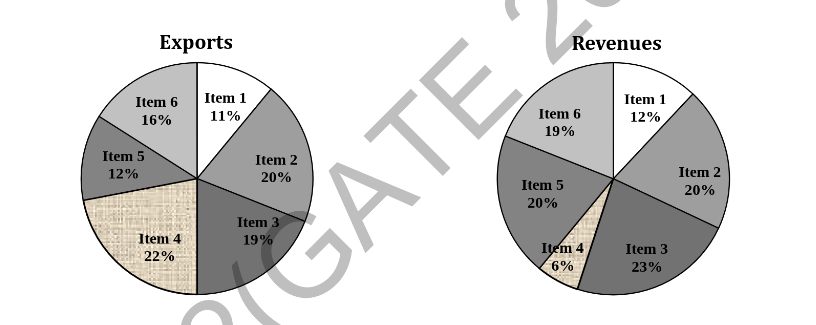
\includegraphics[width=0.5\columnwidth]{figs/01.png} 
    \caption{}
    \label{fig:48}
\end{figure}
\begin{enumerate}
    \item $1:2$
    \item $2:1$
    \item $1:4$
    \item $4:1$
\end{enumerate}

\item X is $1$ km northeast of Y. Y is $1$ km southeast of Z. W is $1$ km west of Z. P is $1$ km south of W. Q is $1$ km east of P. What is the distance between X and Q in km?

\hfill{(GATE GG 2014)}
\begin{enumerate}
    \begin{multicols}{4}
    \item $1$
    \item $\sqrt{2}$
    \item $\sqrt{3}$
    \item $2$
    \end{multicols}
\end{enumerate}

\item 10\% of the population in a town is HIV. A new diagnostic kit for HIV detection is available; this kit correctly identifies HIV individuals 95\% of the time, and HIV individuals 89\% of the time. A particular patient is tested using this kit and is found to be positive. The probability that the individual is actually positive is \makebox[2cm]{\hrulefill}

\hfill{(GATE GG 2014)}\\
\vspace{0.8cm}
\hspace*{4cm}\textbf{END OF THE  QUESTION PAPER }
\end{enumerate}
\begin{enumerate}[start=1]
\item Which one of the following planets has the highest bulk density?

\hfill{(GATE GG 2014)}\\
\begin{multicols}{4}
    \begin{enumerate}
    \item  Jupiter
\item  Venus
\item  Saturn
\item  Mars
\end{enumerate}
\end{multicols}



\item Mid-Oceanic ridges mark plate margins and can be traced by belts of focus earthquakes.

\hfill{(GATE GG 2014)}\\
\begin{multicols}{2}
    \begin{enumerate}
    \item  constructive, shallow
\item  destructive, shallow
\item  constructive, deep
\item  destructive, deep
\end{enumerate}
\end{multicols}


\item  From the surface to the Earth's interior, the velocity of P-wave decreases and the material density increases at the boundary between

\hfill{(GATE GG 2014)}\\
\begin{enumerate}
    \item  Outer core and inner core
\item  Mantle and outer core
\item  Crust and mantle
\item  Upper crust and lower crust
\end{enumerate}


\item The following gamma ray (GR) log data are recorded in a borehole:\\
GR log value against a formation = $30$ API units,\\
Maximum GR log value = $45$ API units,\\
Minimum GR log value = $20$ API units.\\

What is the fraction of shale in the formation?
\hfill{(GATE GG 2014)}\\
\begin{enumerate}
\begin{multicols}{5}
    \item  $0.33$
\item  $0.40$
\item $0.66$
\item $0.75$
\end{multicols}
\end{enumerate}

\item Cirques are formed by

\hfill{(GATE GG 2014)}\\
\begin{multicols}{4}
    \begin{enumerate}
    \item  glaciers
    \item rivers
\item  lakes
\item  oceans
\end{enumerate}
\end{multicols}


\item During which of the following geological eras did birds and mammals first appear on the Earth?

\hfill{(GATE GG 2014)}\\
\begin{multicols}{4}
    \begin{enumerate}
    \item  Cenozoic
\item  Mesozoic
\item  Paleozoic
\item  Proterozoic
\end{enumerate}
\end{multicols}



\item Select the copper ore minerals from the following:

\hfill{(GATE GG 2014)}\\
\hspace*{2cm}(P) Chalcopyrite\\
\hspace*{2cm}(Q) Pyrite\\
\hspace*{2cm}(R) Pyrrhotite\\
\hspace*{2cm}(S) Bornite\\
\hspace*{2cm}(T) sphalerite\\
\hspace*{2cm}(U) chalcocite\\
\begin{enumerate}
    \item  P, S, U
\item  P, Q, R
\item  S, T, U
\item  Q, R, U

\end{enumerate}

\item The reflection coefficient at the interface between two layers of resistivities $9$ \ohm m and $1$ \ohm m respectively is

\hfill{(GATE GG 2014)}\\
\begin{multicols}{2}
    \begin{enumerate}
    \item  $0.6$
\item  $0.7$
\item  $0.8$
\item  $0.9$
\end{enumerate}
\end{multicols}


\item In electromagnetic \brak{EM} sounding, the depth of investigation  with \makebox[1cm]{\hrulefill} increasing frequency.

\hfill{(GATE GG 2014)}\\
\begin{multicols}{2}
    \begin{enumerate}
    \item  increases
\item  decreases
\item  remains unchanged
\item  varies randomly
\end{enumerate}
\end{multicols}


\item  The International Gravity Formula predicts the theoretical gravity value at a given point assuming a

\hfill{(GATE GG 2014)}\\
\begin{enumerate}
    \item  non-rotating homogeneous spherical earth model
\item  rotating inhomogeneous spherical earth model
\item  rotating homogeneous oblate spheroidal earth model
\item  rotating inhomogeneous oblate spheroidal earth model
\end{enumerate}

\item The diurnal variation of geomagnetic elements is due to a system of electric currents flowing in the
\hfill{(GATE GG 2014)}\\
\begin{enumerate}
    \item  ionosphere
\item  Earth's outer core
\item  inter-planetary medium
\item  oceans
\end{enumerate}

\item Match the mineral deposits (listed in Group I) with the most appropriate geophysical exploration methods(listed in Group II)
\hspace*{15.7cm}{(GATE GG 2014)}\\
\begin{tabular}{ l l }
\textbf{Group I} & \textbf{Group Il}\\
(P) Mineralized conductive veins & (1)Gravity\\
(Q) Disseminated sulphides & (2)Magnetic\\
(R) Massive barytes & (3)Induced Polarization\\
(S) Kimberlite pipes & (4) Resistivity profiling\\
 & (5) Low frequency Magnetotellurics
 \end{tabular}
 \begin{multicols}{2}
     \begin{enumerate}
    \item  P-4; Q-3; R-1; S-5
    \item  P-2; Q-1; R-4; S-5
    \item P-5; Q-1; R-4; S-3
    \item P-4; Q-3; R-1; S-2
\end{enumerate}
 \end{multicols}


\item  In seismic refraction surveys, the critical distance

\hfill{(GATE GG 2014)}\\
\begin{enumerate}
    \item is always less than the crossover distance
\item  is always more than the crossover distance
\item  is always equal to the crossover distance
\item  cannot be compared with the crossover distance

\end{enumerate}

\item As compared to large earthquakes, small earthquakes are

\hfill{(GATE GG 2014)}\\
\begin{enumerate}
    \item  more frequent and caused by short fault slip and long rupture lengths
\item  more frequent and caused by long fault slip and short rupture lengths
\item  less frequent and caused by short fault slip and short rupture lengths
\item  more frequent and caused by short fault slip and short rupture lengths
\end{enumerate}

\item  Match the type of well logs (listed in Group I) with the characteristics of measurement (listed in Group II).\\

\hfill{(GATE GG 2014)}\\
\begin{tabular}{ l l }
\textbf{Group I} & \textbf{Group Il}\\
(P) Dipmeter & (1) Hydrogen concentration in pores\\
(Q) Neutron & (2) Velocity of compressional waves\\
(R) SP & (3) Correlation of resistivity changes\\
(S) Sonic & (4) Natural radioactivity\\
 & (5) Natural electric potential
 \end{tabular}
 \begin{multicols}{2}
     \begin{enumerate}
    \item  P-3; Q-1; R-5; S-2
    \item  P-4; Q-1; R-5; S-3
    \item  P-3; Q-4; R-5; S-2
\item  P-3; Q-1; R - 4; S-2
\end{enumerate}
 \end{multicols}


\item For earthquakes of magnitudes $6$ and $7$, the seismic wave amplitudes are $A_6$ and $A_7$ energies are $E_6$ and $E_7$ respectively.

Which one of the following is true?

\hfill{(GATE GG 2014)}\\
\begin{enumerate}
    \item  $A_7$ $=$ $(7/6)$ $A_6$ and $E_7$$=$ $10$ $E_6$
\item  $A_7$ $=$ $10$ $A_6$ and $E_7$$=$ $100$ $E_6$
\item  $A_7$ $=$ $10$ $A_6$ and $E_7$$=$ $(7/6)$ $E_6$
\item  $A_7$ $=$ $10$ $A_6$ and $E_7$$=$ $32$ $E_6$
\end{enumerate}

\item  Structure contours of a bedding plane at $100$ m interval are spaced in such a manner that the horizontal equivalent is also $100$m. The dip of the bedding plane is

\hfill{(GATE GG 2014)}\\
\begin{multicols}{4}
    \begin{enumerate}
    \item $30\degree$
     \item $45\degree$
     \item $60\degree$
      \item $90\degree$
\end{enumerate}
\end{multicols}


\item Horizontal slickensides are observed on the surface of a vertical fault. What is the type of fault?

\hfill{(GATE GG 2014)}\\
\begin{multicols}{4}
    \begin{enumerate}
\item  Normal fault
\item Reverse fault
\item  Strike-slip fault
\item  Oblique fault
\end{enumerate}
\end{multicols}


\item Match the mineral habits(listed in Group I)with the minerals (listed in Group II)

\hfill{(GATE GG 2014)}\\
\begin{tabular}{ l l }
\textbf{Group I} & \textbf{Group Il}\\
 (P)Acicular & (1) Kyanite\\
(Q) Fibrous  & (2) Beryl\\
(R) Bladed & (3) Sillimanite\\
(S) Columnar & (4)Chrysotile\\
 & (5)Olivine
 \end{tabular}
 \begin{multicols}{2}
     \begin{enumerate}
    \item P-3; Q-2; R-5; S-1
    \item P-4; Q-5; R-1; S-2
    \item P-2; Q-3; R-4; S-1
    \item P-3; Q-4; R-1; S-2
\end{enumerate}
 \end{multicols}


\item  The correct chronological order (older to younger) of the following volcanic events is

\hfill{(GATE GG 2014)}\\
(P) Rajmahal volcano

(Q) Deccan volcanism

(R) Panjal volcanism

(S) Malani volcanism


\begin{enumerate}
    \item  P, Q, R, S
    \item S, R, Q, P
\item  S, R, P, Q
\item  S, Q, R, P
\end{enumerate}


\item A clastic rock dominantly composed of feldspar grains is

\hfill{(GATE GG 2014)}\\
\begin{multicols}{4}
    \begin{enumerate}
    \item  shale
\item  arenite
\item  greywacke
\item  arkose
\end{enumerate}
\end{multicols}



\item A metamorphic rock consists of pyroxene, plagioclase and quartz, and exhibits hornfelsic texture.The rock has undergone \makebox[2cm]{\hrulefill} metamorphism.

\hfill{(GATE GG 2014)}\\
\begin{multicols}{4}
    \begin{enumerate}
    \item  regional
\item  contact
\item  cataclastic
\item  impact
\end{enumerate}

\end{multicols}

\item An igneous body with a flat top and a concave-upward base is known as a

\hfill{(GATE GG 2014)}\\
\begin{multicols}{4}
    \begin{enumerate}
    \item  laccolith
\item  lopolith
\item  sill
\item  stock
\end{enumerate}
\end{multicols}


\item The velocity discontinuity between the upper crust and the lower crust is known as \makebox[2cm]{\hrulefill} discontinuity.

\hfill{(GATE GG 2014)}\\
\begin{multicols}{2}
    \begin{enumerate}
    \item Lehman
    \item Gutenberg
    \item Mohorovicic
    \item Conard
\end{enumerate}
\end{multicols}


\item Match the items listed in Group I with those in Group II

\hfill{(GATE GG 2014)}\\
\begin{tabular}{ l l }
\textbf{Group I} & \textbf{Group Il}\\
(P) Isopachs & (1) Contours of equal slope\\
(Q) Isotherms & (2) Contours of equal thickness\\
(R) Isochrons & (3) Contours of equal temperature\\
(S) Isotans & (4) Contours of equal core thickness\\
 & (5) Contours of equal age
 \end{tabular}
 \begin{multicols}{2}
     \begin{enumerate}
    \item  P-2; Q-3; R-1; S-5
\item  P-2; Q-3; R-5; S-1
\item P-1; Q-3; R-2; S-4
\item P-5; Q-4; R-3; S-1
\end{enumerate}
 \end{multicols}

\vspace{5cm}
\textbf{PART B (SECTION 1): FOR GEOLOGY CANDIDATES ONLY}
\item Match the items in Group I with those in Group II

\hfill{(GATE GG 2014)}\\
\begin{tabular}{ l l }
\textbf{Group I} & \textbf{Group Il}\\
(P) Interference colour & (1) Property of a single grain seen under microscope in polarized light\\

(Q)Twinkling & (2) Property of a single grain seen under microscope under crossed nicols\\

(R) Pleochroism & (3) Property seen when several grains are viewed collectively under microscope in polarized light\\

(S) Play of colours & (4) Property of a mineral seen in hand specimen
\end{tabular}
\begin{multicols}{2}
    \begin{enumerate}
    \item  P-2; Q-3; R-1; S-4
    \item P-2; Q-3; R-4; S-1
    \item P-3; Q-4; R-1; S-2
    \item P-1; Q-4; R-2; S-3
\end{enumerate}
\end{multicols}


\item Which one of the following represents a closed crystallographic form?

\hfill{(GATE GG 2014)}\\
\begin{multicols}{2}
    \begin{enumerate}
    \item  Hexagonal prism
\item Hexagonal dipyramid
\item  Tetragonal pyramid
\item Ditetragonal prism

\end{enumerate}
\end{multicols}


\item In the figure given below a, b and c are the crystallographic axes of a crystal. The Miller Index of the crystal face PQR is:
\begin{figure}[H]
    \centering
    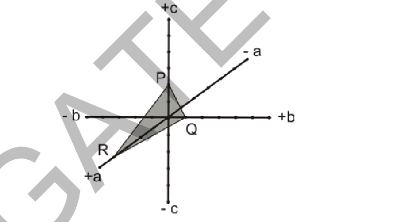
\includegraphics[width=0.5\columnwidth]{figs/02.png} 
    \caption{}
    \label{fig:48}
\end{figure}

\hfill{(GATE GG 2014)}\\
\begin{enumerate}
\begin{multicols}{4}
     \item $\brak{421}$
    \item $\brak{124}$
    \item $\brak{142}$
    \item $\brak{214}$
\end{multicols}
\end{enumerate}

\item Match the alkaline rocks listed in Group I with their characteristics listed in Group II

\hfill{(GATE GG 2014)}\\
\begin{tabular}{ l l }
\textbf{Group I} & \textbf{Group Il}\\
(P) Basanite & (1) Volcanic rock lacking feldspar\\

(Q) Nephelinite & (2) Ultrapotasic volcanic rock\\

(R) Shonshonite & (3) Feldspathoid-bearing basalt\\

(S) Lamproite & (4) K-rich basalt\\
\end{tabular}
\begin{multicols}{2}
\begin{enumerate}
    \item  P-4; Q-1; R-3; S-3
\item  P-1; Q-2; R-3; S-4
\item  P-3; Q-1; R-4; S-2 
\item  P-2; Q-1; R-4; S-3
\end{enumerate}
\end{multicols}

\item  In a metamorphic terrain, crenulations at the hinge zone of a fold along with the development of axial plane foliation is an evidence of
\hfill{(GATE GG 2014)}
\begin{enumerate}
    \item  one phase of deformation
\item  at least two phases of deformation
\item  no deformation
\item  extensional regime of the deformation
\end{enumerate}

\item A phase-diagram with a specified bulk-composition is known as
\hfill{(GATE GG 2014)}
\begin{multicols}{4}
    \begin{enumerate}
        \item  isograd diagram
\item  AFM diagram
\item  pseudosection
\item  ACF diagram
    \end{enumerate}
\end{multicols}

\item The uniaxial interference figure of a mineral given below shows the changes in the position of color bands when a mica plate is inserted in the accessory slot of the microscope as shown. The changes in the interference figure are due to\\
\hspace*{15.7cm}(GATE GG 2014)
\begin{figure}[H]
    \centering
    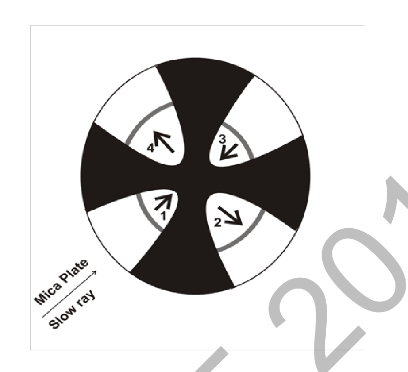
\includegraphics[width=0.5\columnwidth]{figs/03.png} 
    \caption{}
    \label{fig:48}
\end{figure}
\begin{enumerate}
    \item  increase in retardation along the quadrants 1 and 3
\item  increase in retardation along the quadrants 2 and 4
\item  decrease in retardation along the quadrants 1 and 3
\item  increase in retardation in all quadrants

\end{enumerate}

\item The relative enrichment factors ($\triangle$ values) of sulphur isotopes of two sulphide minerals A and B in equilibrium with H$_2$S at the same P-T-X conditions are $+5.9\%$ and $-11.2\%$ respectively. If A and B are in equilibrium under the same P-T-X conditions and $\delta^{34}\delta$ value of A is +6.8\%, then the $\delta^{34}\delta$ value of B is
\hfill(GATE GG 2014)

    \begin{enumerate}
    \item  $-10.3\%$
\item  $+10.3\%$
\item $-9.3\%$
 \item $+9.3\%$
\end{enumerate}

\vspace{0.5cm}

\item If $\mathrm{Fe^{2+} \rightarrow Fe^{3+} + e^-}$, $E^\circ = +0.77 \ \mathrm{volt}$, $E_h = 0.6 \ \mathrm{volt}$,K=$\frac{[\mathrm{Fe^{3+}}]}{[\mathrm{Fe^{2+}}]}$and the basic equation to be used is:$E_h=E^\circ +\frac{0.059}{n}\log k$ Then the value of $\frac{\mathrm{Fe^{2+}}}{\mathrm{Fe^{3+}}}$  in the solution is \underline{\hspace{1.5cm}} 
\hfill(GATE GG 2014)
\vspace{0.5cm}

\item  In an ore mine exposing stratified sulfide ore with sulfide bands having thickness between $10$ and $100$ cm, which one of the following sampling methods is the most appropriate?
\hfill(GATE GG 2014)

\begin{enumerate}

    \item Chip sampling
    \item Channel sampling
    \item Bulk sampling
    \item Grab sampling
\end{enumerate}

\item From the given Eh-pH diagram, which one of the following pairs can be inferred to be a disequilibrium assemblage?\\
\hspace*{15.7cm}(GATE GG 2014)
\begin{figure}[H]
    \centering
    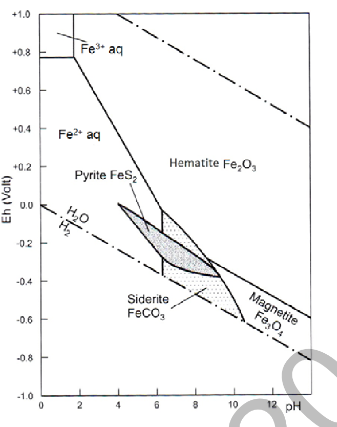
\includegraphics[width=0.26\columnwidth]{figs/04.png} 
    \caption{}
    \label{fig:48}
\end{figure}
\begin{multicols}{2}
\begin{enumerate}
    \item Hematite-magnetite
    \item Magnetite-Pyrite
    \item Pyrite-siderite
    \item Hematite-siderite
\end{enumerate}
\end{multicols}

\item Metal content (in metric tonnes) of an ore having specific gravity and assay values of $2.86$ and $1.49\%$ respectively in a mining block $40$ m long, $30$ m wide and with an average thickness of $2.13$ m is\underline{\hspace{1.5cm}} 
\hfill(GATE GG 2014)
\vspace{0.5cm}
\item From the list of planktic foraminifera below, the pair having a supplementary sutural aperture is\\
\brak{P}Globineria\\
\brak{Q}Globorotilia\\
\brak{R}Globigerinoides\\
\brak{S}Orbulina
\hfill(GATE GG 2014)
\begin{multicols}{2}
\begin{enumerate}
    \item P, Q
    \item Q, R
    \item P, R
    \item R, S
\end{enumerate}
\end{multicols}

\item Match the morphological features (listed in Group I) with their corresponding fuels (listed in Group II) 

\hfill{(GATE GG 2014)}\\
\begin{tabular}{ l l }
\textbf{Group I} & \textbf{Group Il}\\
P. Axial lobe & 1. Graptolite \\
Q. Coiled chambers & 2. Gastropod \\
R. Colonial corallites & 3. Conodont \\
S. Conical shell & 4. Foraminifer \\
 & 5. Trilobite \\
 & 6. Coral \\
 \end{tabular}
 \begin{multicols}{2}
 \begin{enumerate}
\item P-2; Q-3; R-1; S-6 
\item  P-5; Q-3; R-1; S-2 
\item P-3; Q-1; R-4; S-2 
\item P-2; Q-3; R-4; S-6 
 \end{enumerate}
\end{multicols}

\item Which one of the following marine environments is indicated by the assemblage of benthic foraminifera $Quinqueloculina, Lenticulina, Ammonia, Elphidium$?
\hfill(GATE GG 2014)
\begin{multicols}{2}
\begin{enumerate}
    \item Abyssal
    \item Bathyal
    \item Shelf
    \item Hadal
\end{enumerate}
\end{multicols}

\item The correct chronological order (older to younger) of the following geological units is:
\hfill(GATE GG 2014)\\
 \brak{P}Talchir Tillite\\
\brak{Q}Muth Quartzite\\
\brak{R}Umia Ammonites Bed\\
 \brak{S}Umaria Marine Bed\\

\begin{enumerate}
    \item P -- R -- S -- Q
    \item Q -- P -- S -- R
    \item R -- Q -- P -- S
    \item P -- Q -- R -- S
\end{enumerate}

\item The best match of terms in \textbf{Group I} with those in \textbf{Group II} is:
\hfill{(GATE GG 2014)}\\
\begin{tabular}{ l l }
\textbf{Group I} & \textbf{Group Il}\\
P. Alkali reaction & 1. Tunneling in hard rocks\\
Q. Arching & 2. Earth dam\\
R. Rip rap & 3.Slope protection\\ 
S. Clay core & 4.Gravity dam\\
\end{tabular}
\begin{multicols}{2}
\begin{enumerate}
    \item P-4; Q-5; R-1; S-3
     \item P-5;Q-4;R-2;S-3
     \item P-3; Q-1; R-4; S-2
     \item P-1; Q-3; R-4; S-2
\end{enumerate}
\end{multicols}

\item Knick points indicate change in the 
\hfill(GATE GG 2014)
\begin{enumerate}
    \item attitude of beds
    \item strike of a fault
    \item attitude of joints
    \item stream gradient 
\end{enumerate}

\item A confined sandy aquifer has a thickness of $10$m and transmissivity of $0.75$m$^2$per day. Its hydraulic conductivity is;\\
\hspace*{15.7cm}(GATE GG 2014)

\vspace{0.5cm}

\item A geological reconnaissance survey is being carried out using remote sensing multispectral data. Which set of the two band data of the following is most appropriate for mapping limonite bearing zones? 
\hfill(GATE GG 2014)
\begin{enumerate}
    \item Near infrared band and Thermal infrared band image data 
\item  Visible band and Near infrared band image data 
\item  Shortwave infrared band and Thermal infrared image data 
\item  Thermal infrared band and X-band radar image data
\end{enumerate}

\item The maximum amount of hydrogen (dry mineral matter free basis) in bituminous-anthracite is:  
\hfill(GATE GG 2014)
\begin{multicols}{2}
   \begin{enumerate}
       \item less than 10\% 
\item  10--15\% 
\item  15--20\% 
\item  20--25\%
\end{enumerate}
\end{multicols}

\item The standard free energy change (in kJ) at \( 25^\circ \mathrm{C} \) of the dissolution of anhydrite at equilibrium in the equation $\mathrm{CaSO_4 \; \rightleftharpoons \; Ca^{2+} + SO_4^{2-}}$,given \( K = 3.4 \times 10^5 \) and \( R = 8.314 \ \mathrm{J/mol/K} \), is:
\hfill(GATE GG 2014)
\begin{multicols}{4}
    \begin{enumerate}
    \item $43.7$
    \item $37.4$
    \item $30.2$
    \item $25.5$
\end{enumerate}
\end{multicols}

\item 
\begin{figure}[H]
    \centering
    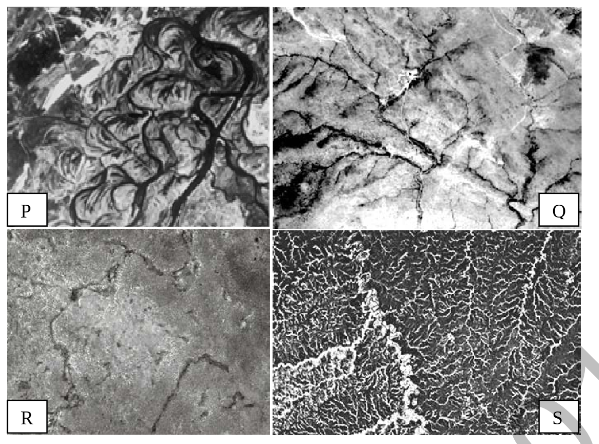
\includegraphics[width=0.5\columnwidth]{figs/05.png} 
    \caption{}
    \label{fig:48}
\end{figure}
Drainage patterns observed in four areas are shown in black-and-white panchromatic images P,Q,R,S. Field work in these areas has indicated presence  of the following lithology/geological unit?  
\hfill(GATE GG 2014)\\
1. Fractured quartzite\\  
2. Shale\\
3. Limestone\\  
4. Alluvial plain\\  
The correct match of the drainage patterns with the lithology/geological unit is
\begin{enumerate}
    \item P-1; Q-2; R-4; S-3
    \item P-4; Q-1; R-3; S-2
    \item P-4; Q-1; R-2; S-3
    \item P-2; Q-1; R-3; S-4
\end{enumerate}


\item 
\begin{figure}[H]
    \centering
    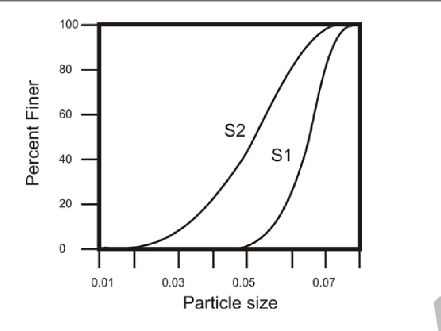
\includegraphics[width=0.5\columnwidth]{figs/06.png} 
    \caption{}
    \label{fig:48}
\end{figure}
The given figure shows the grain size distribution of two soil samples S1 and S2.  
The uniformity coefficient is defined as \( U = d_{60} / d_{10} \), where \( d_{60} \) and \( d_{10} \) represent particle sizes corresponding to 60 and 10 percent  finer, respectively. Determine the correctness or otherwise of the Assertion (a) and Reason (r)\\
Assertion (a): S1 has a higher value of uniformity coefficient than S2.\\ 
Reason (r): S1 has less variation in grain-size than S2.
\hfill(GATE GG 2014)
\begin{enumerate}
    \item Both (a) and (r) are true, and (r) is the correct reason for (a).
    \item Both (a) and (r) are false.
    \item (a) is false but (r) is true, (r) being not the correct reason for(a).
    \item (a) is true but (r) is false.
\end{enumerate}

\item The geological map given below shows beds in a normal stratigraphic order. Which one of the following statements is true in respect of features near locations P and Q?
\hfill(GATE GG 2014)
\begin{figure}[H]
    \centering
    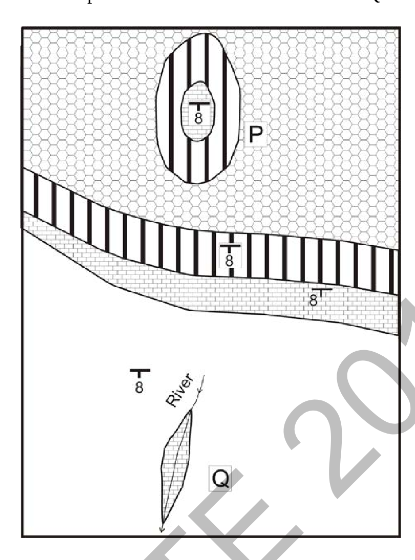
\includegraphics[width=0.32\columnwidth]{figs/07.png} 
    \caption{}
    \label{fig:48}
\end{figure}
\begin{enumerate}
    \item P is an anticline and Q is a syncline
    \item Q is an anticline and P is a syncline
    \item P is an outlier and Q is an inlier
    \item Q is an outlier and P is an inlier
\end{enumerate}

\item Four aqueous-vapor fluid inclusions P, Q, R and S are petrographically identical at room temperature, and contain approximately 90\% liquid and 10\% vapor. The freezing temperatures of the fluid inclusions are:  $P = -5.3\, ^\circ\text{C},  Q = -16.6\, ^\circ\text{C},  R = -21.2\, ^\circ\text{C},  S = -8.7\, ^\circ\text{C}$
With respect to P, Q, R and S, the correct statement is:
\hfill(GATE GG 2014)
\begin{enumerate}
    \item salinity of p is highest but density is lowest
    \item both salinity and density of Q are lowest
    \item both salinity and density of R are highest
    \item both salinity and density of S are lowest
\end{enumerate}

\item Which one of the following is the youngest marine formation in the Himalaya?  
\hfill(GATE GG 2014)
\begin{multicols}{2}
\begin{enumerate}
    \item Dagshahi Formation
    \item Subathu Formation
    \item Kasauli Formation
    \item Karewa Formation
\end{enumerate}
\end{multicols}

\item Which one of the following environments is represented by molasse facies?
\hfill(GATE GG 2014)\begin{multicols}{2} 
\begin{enumerate}
    \item Atectonic
    \item Pre-tectonic
    \item Syn-tectonic
    \item Post-tectonic
\end{enumerate}
\end{multicols}

\item In the given ternary diagram (Fo = forsterite; Di = diopside; An = anorthite) eutectic diagram, the point A represents the composition of magma.  
What will be the sequence of crystallization during cooling of this magma?
\hfill(GATE GG 2014)
\begin{figure}[H]
    \centering
    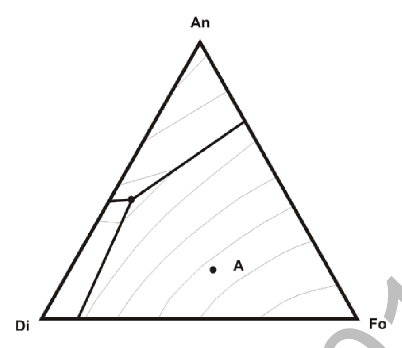
\includegraphics[width=0.5\columnwidth]{figs/08.png} 
    \caption{}
    \label{fig:48}
\end{figure}
\begin{enumerate}
    \item olivine and olivine$+$plagioclase
    \item olivine and olivine$+$pyroxene
    \item olivine,olivine$+$plagioclase and olivine$+$plagioclase$+$pyroxene
    \item olivine,olivine$+$pyroxene and olivine$+$pyroxene$+$plagioclase
\end{enumerate}

\item Which one of the following is the best suited mining method for a low-dipping, tabular-shaped, hard and compact ore body with $2$ to $2.5$m thickness sandwiched between hard and compact roof and floor rock?
\hfill(GATE GG 2014)
\begin{multicols}{2}
    \begin{enumerate}
    \item Cut and fill method
    \item Shrinkage stope method
    \item Open stope method
    \item Caving method
\end{enumerate}
\end{multicols}
\vspace{0.6cm}
\textbf{PART B (SECTION 2): FOR GEOPHYSICS  CANDIDATES ONLY}
\end{enumerate}
\begin{enumerate}[start=26]
    \item A gaseous hydrocarbon-bearing zone can be best identified by a combined analysis of:
    
\hfill(GATE GG 2014)
\begin{enumerate}
    \item Density and Self potential (SP) logs
    \item Density and Neutron logs
    \item Sonic and Neutron logs
    \item Natural gamma ray (GR) and Neutron logs
\end{enumerate}

\item In general, geophysical inverse problems dealing with real data obtained from field measurements are:

\hfill(GATE GG 2014)
\begin{multicols}{2}
    \begin{enumerate}
    \item grossly over determined
    \item even determined
    \item over determined
    \item grossly underdetermined
\end{enumerate}
\end{multicols}

\item In vector calculus, Stoke's theorem relates:

\hfill(GATE GG 2014)
\begin{multicols}{2}
    \begin{enumerate}
    \item line-integral to volume integral
    \item surface integral to volume integral
    \item scalar product integral to norm
    \item line integral to surface integral
\end{enumerate}
\end{multicols}

\item The radial dependence of the solution of the Laplace equation in cylindrical coordinates is expressed in terms of:

\hfill(GATE GG 2014)
\begin{multicols}{2}
    \begin{enumerate}
    \item Bessel function
    \item Legendre polynomial
    \item Exponential function
    \item Hermite polynomial
\end{enumerate}
\end{multicols}

\item For an electrostatic field, the Maxwell's equations reduce to:

\hfill(GATE GG 2014)
\begin{multicols}{2}
    \begin{enumerate}
    \item Wave equation
    \item Diffusion equation
    \item Helmholtz equation
    \item Poisson equation
\end{enumerate}
\end{multicols}

\item Which one of the following functions is used as a source-term to obtain the Green's function of a boundary value problem?

\hfill(GATE GG 2014)
\begin{multicols}{2}
    \begin{enumerate}
    \item Heaviside unit step function
    \item Exponential function
    \item Rectangular function
    \item Dirac delta function
\end{enumerate}
\end{multicols}

\item The heat flow through a unit area of the Earth's surface is given by the product of:

\hfill(GATE GG 2014)
\begin{enumerate}
    \item vertical thermal gradient and thermal conductivity
    \item horizontal thermal gradient and thermal conductivity
    \item vertical thermal gradient and thermal diffusivity
    \item horizontal thermal gradient and thermal diffusivity
\end{enumerate}

\item The S-wave velocity of a medium having a Poisson's ratio and a P-wave velocity of $0.5$ and $3$km/s respectively is \underline{\hspace{2cm}}km/s.

\hfill(GATE GG 2014)
\item The PKiKP phase denotes the passage of a seismic wave in the Earth as:

\hfill(GATE GG 2014)
\begin{enumerate}
    \item P in mantle, S in outer core, reflected as P from inner outer core, boundary S in outer core ,P in mantle and crust
    \item P in crust, P in mantle, reflected as P from core mantle boundary, P in mantle, P in crust
    \item P in mantle, P in outer core, P in inner core, P in outer core, P in mantle and crust
    \item P in mantle, P in outer core, reflected as P from inner outer core boundary, P in outer core, P in mantle and crust
\end{enumerate}


\item Match the items of \textbf{Group I} with those in \textbf{Group II}:
\hfill{(GATE GG 2014)}\\
\begin{tabular}{ l l }
\textbf{Group I} & \textbf{Group Il}\\
(P) proton precission magnetometer & Induction in a pair of high permeable cores\\
(Q) Alkali vapor magnetometer & SQUID\\
(R) Fluxgate magnetometer & Radio spectroscopy\\
(S) Superconducting magnetometer & Nuclear magnetic resonance\\
\end{tabular}
\begin{multicols}{2}
\begin{enumerate}
 \item P-2; Q-3; R-4; S-1
     \item P-4;Q-3;R-1;S-2
     \item P-4; Q-1; R-3; S-2
     \item P-4; Q-2; R-1; S-3
\end{enumerate}
\end{multicols}

\item Konigsberger ratio refers to:

\hfill(GATE GG 2014)
\begin{enumerate}
    \item anisotropy of magnetic susceptibility
    \item ratio of remanent magnetization and induced magnetization
    \item ratio of longitudinal and transverse electrical resistivities
    \item ratio of P and S wave velocities
\end{enumerate}

\item The Poisson's relation linking the gravity and magnetic potentials assumes the same anomaly source with:

\hfill(GATE GG 2014)
\begin{enumerate}
    \item inhomogeneous density and intensity of magnetization
    \item uniform density contrast and inhomogeneous intensity of magnetization
    \item uniform density contrast and homogeneous intensity of magnetization
    \item inhomogeneous density and homogeneous intensity of magnetization
\end{enumerate}

\item Compute the coefficient of anisotropy from the following parameters estimated from a Vertical Electric Sounding (VES) survey:  

\hfill(GATE GG 2014)\\
Resistivity of first layer, $\rho_1 = 15 \ \Omega-$m\\  
Resistivity of second layer, $\rho_2 = 4 \ \Omega-$m\\  
Resistivity of lower half-space, $\rho_3 = 50 \ \Omega-$m\\  
Thickness of first layer, $h_1 = 3 m$\\  
Thickness of second layer, $h_2 = 16m$\\  
\begin{enumerate}
    \item $1.43$
    \item $1.28$
    \item $1.19$
    \item $1.12$
\end{enumerate}

\item The convolution of two finite length sequences $x_n = \sbrak{1, 0, -2}$ and $y_n = \sbrak{1, -1}$ is
\hfill(GATE GG 2014)
\begin{enumerate}
    \item \sbrak{-1, 1, 2, -2}
    \item \sbrak{1, -1, -2, 2}
    \item \sbrak{1, 0, -2, 2}
    \item \sbrak{-1, 0, -2, 1}
\end{enumerate}

\item Arrange the following electrode configurations in the ascending order of their depth of investigation:
\hfill(GATE GG 2014)\\
 Dipole-- Dipole\\  
  Schlumberger\\  
  Wenner\\  
  Pole--Pole\\  
\begin{enumerate}
\item R--S-Q-p
\item P--Q-S-R
\item R--Q-P-S
\item R--Q-S-P
 \end{enumerate}

 \item Which one of the following transforms relates the real and imaginary components of harmonic functions?
 \hfill(GATE GG 2014)
\begin{multicols}{2}
    \begin{enumerate}
    \item Hilbert transform
    \item Laplace transform
    \item Fourier transform
    \item Wavelet transform
\end{enumerate}
\end{multicols}

\item Which one of the following geophysical methods is most suitable for exploration of possible hydrocarbon-bearing sediments underlying the Deccan Traps?

\hfill(GATE GG 2014)
\begin{multicols}{2}
    \begin{enumerate}
    \item Seismic
    \item Magnetotellurics
    \item DC resistivity
    \item Airborne EM
\end{enumerate}
\end{multicols}

\item A collection of traces having a common mid-point is called a CMP gather. The number of traces in an $n$-fold survey in a CMP gather is:

\hfill(GATE GG 2014)
\begin{multicols}{4}
    \begin{enumerate}
    \item n-1
    \item  n + 1
    \item  n 
    \item  $\frac{n}{2}$ 
\end{enumerate}
\end{multicols}

\item In seismic prospecting, migration is the process of moving data elements from:

\hfill(GATE GG 2014)
\begin{enumerate}
    \item midpoint locations to subsurface locations
    \item subsurface locations to midpoint locations
    \item midpoint locations to surface locations
    \item subsurface locations to surface locations
\end{enumerate}

\item An $80$ Hz seismic signal is sampled at a rate of $100$ samples/s. What will be its aliased period \brak{in seconds} in the sampled signal?

\hfill(GATE GG 2014)
\begin{multicols}{4}
    \begin{enumerate}
    \item 30
    \item 10
    \item 0.1
    \item 0.05
\end{enumerate}
\end{multicols}

\item The Fourier transform and integral of the Dirac delta function respectively are:

\hfill(GATE GG 2014)
\begin{multicols}{2}
   \begin{enumerate}
    \item 1 and 1
    \item 0 and 0
    \item 0 and 1
    \item 1 and $\infty$
\end{enumerate} 
\end{multicols}

\item A signal $x_n = [2, 1]$ is input to a system whose impulse response is $h_n = [8, 4, 2, 1]$.
The $z$-transform of the output is:

\hfill(GATE GG 2014)
\begin{enumerate}
    \item $16 + 16 z^{-1} + 3 z^{-2} + 4 z^{-3} + z^{-4}$
    \item $10 + 5 z^{-1} + 2 z^{-2} + 4 z^{-3} + z^{-4}$
    \item $16 + 16 z^{-1} + 8 z^{-2} + 4 z^{-3} + z^{-4}$
    \item $16 + 16 z + 8 z^{-2} + 2 z^{-3} + z^{-4}$
\end{enumerate}

\item Calculate the formation water saturation, $S_w$, from the following well log data: Resistivity of completely saturated formation, $R_0 = 1.8\ \Omega \cdot$m .True resistivity of formation, $R_t = 25\ \Omega \cdot$m  
\hfill(GATE GG 2014)
\begin{multicols}{2}
    \begin{enumerate}
    \item 31\%
    \item 29\%
    \item 27\%
    \item 25\%
    \end{enumerate}
\end{multicols}

\item Consider the four systems of algebraic equations (listed in Group I).  
The systems (Q), (R), and (S) are obtained from (P) by restricting the accuracy of data or coefficients or both, respectively, to two decimal places.  
\hfill{(GATE GG 2014)}\\
\begin{tabular}{ l l }
\textbf{Group I} & \textbf{Group Il}\\
(P) $x + 1.0000y = 2.0000$\\$x + 1.0001y = 2.0001$  & (1) Instability \\ 
(Q) $x + 1.0000y = 2.00$\\ $x + 1.0001y = 2.00$  & (2) Inconsistency \\ 
(R) $x + 1.00y = 2.0000$\\$x + 1.00y = 2.0001$ & (3) Non-uniqueness\\
(S)$x + 1.00y = 2.00$\\$x + 1.00y = 2.00$ & (4) Exact   
\end{tabular}
\begin{multicols}{2}
    \begin{enumerate}
         \item P-1; Q-4; R-3; S-2
    \item P-4; Q-1; R-2; S-3
    \item P-4; Q-1; R-3; S-2
    \item P-1; Q-4; R-2; S-3
    \end{enumerate}
\end{multicols}

\item The eigenvalue ($\Lambda$) and eigenvector (U) matrices for singular value decomposition of the matrix $\begin{pmatrix}
    2 & 1 \\
    2 & 0
\end{pmatrix}$ respectively are:\\
\hspace*{15.7cm}(GATE GG 2014)
\begin{multicols}{2}
\begin{enumerate}
    \item $\Lambda=\begin{pmatrix}
        3 & 0\\
        0 & 1
    \end{pmatrix}$ and U=$\frac{1}{\sqrt{2}}\begin{pmatrix}
        1 & -1\\
        1 & 1
    \end{pmatrix}$
    \item $\Lambda=\begin{pmatrix}
        3 & 0\\
        0 & 1
    \end{pmatrix}$ and U=$\frac{1}{\sqrt{2}}\begin{pmatrix}
        1 & -1\\
        1 & -1
    \end{pmatrix}$
    \item $\Lambda=\begin{pmatrix}
        2 & 0\\
        0 & 2
    \end{pmatrix}$ and U=$\frac{1}{\sqrt{2}}\begin{pmatrix}
        1 & -1\\
        1 & 1
    \end{pmatrix}$
    \item $\Lambda=\begin{pmatrix}
        2 & 0\\
        0 & 2
    \end{pmatrix}$ and U=$\frac{1}{\sqrt{2}}\begin{pmatrix}
        1 & 1\\
        1 & 1
    \end{pmatrix}$
\end{enumerate}
\end{multicols}

\item The amplitude spectrum of a band pass filter, $A_B$, can be obtained by a combination of spectra of a low pass filter, $A_L$, and that of a high pass filter, $A_H$, as:
\hfill(GATE GG 2014)
\begin{multicols}{2}
    \begin{enumerate}
    \item $A_B = A_L \times A_H$
    \item$ A_B = A_L + A_H $
    \item $ A_B = A_L - A_H $
    \item $ A_B = \frac{A_L}{A_H} $
\end{enumerate}
\end{multicols}

\item Compute the maximum value of gravity anomaly in $\mu$Gal over a buried sphere from the following data: 
\hfill(GATE GG 2014)\\
Radius of a sphere = $5$m \\
Density contrast $0.1$gm/cc \\
Depth to centre of sphere = $11$m \\
G=$6.673\times10^{-8}$dyne-cm$^2$/gm$^2$
\begin{multicols}{4}
    \begin{enumerate}
    \item $2887.58$
    \item $288.76$
    \item $28.88$
    \item $2.89$
\end{enumerate}
\end{multicols}

\item Given the potential field anomaly data at the datum level  z = 0 , match the spatial frequency expressions \brak{\text{listed in Group I}} with the corresponding operations \brak{\text{listed in Group II}}.\brak{ \text{k  is wave number}}
\hfill{(GATE GG 2014)}\\
\begin{tabular}{ l l }
\textbf{Group I} & \textbf{Group Il}\\
(P) exp\brak{\text{-zk}} & (1)Second vertical derivative at the datum level\\
(Q) $k$exp\brak{\text{-zk}} & (2) Analytic continuation into upper half-space\\
(R) $k^2$ & (3)Analytic continuation into lower half-space\\
(S) $k$exp\brak{\text{zk}} & (4)  First vertical derivative of upward continued values\\
 & (5) First vertical derivative of downward continued values
\end{tabular}
\begin{multicols}{2}
    \begin{enumerate}
        \item P-3; Q-3; R-2; S-5
    \item P-2; Q-1; R-4; S-3
    \item P-2; Q-4; R-1; S-3
    \item P-3; Q-1; R-5; S-2
    \end{enumerate}
\end{multicols}

\item \textbf{Assertion (a):} An efficient marine seismic survey should use an implosive source. \\
\textbf{Reason (r):} The performance of a marine seismic source is rated by high pulse-to-bubble ratio.

\hfill(GATE GG 2014)
\begin{enumerate}
    \item Both (a) and (r) are true and (r) is the correct reason for (a)
    \item Both (a) and (r) are true but (r) is not the correct reason for (a)
    \item (a) is true but (r) is false
    \item (a) is false but (r) is true
\end{enumerate}

\item The electric field intensity vector \brak{\text{E}} and the displacement vector \brak{\text{D}} are given by $\brak{E} = 2 \, \hat{\imath} + 2 \, \hat{\jmath} + 4 \, \hat{k} \text{and}  \brak{D} = \hat{\imath} + \hat{\jmath} + \hat{k}$
The energy of the field is:
\hfill(GATE GG 2014)
\begin{multicols}{2}
    \begin{enumerate}
    \item 2
    \item 4
    \item 6
    \item 8
\end{enumerate}
\end{multicols}
\vspace{0.6cm}
\textbf{END OF THE QUESTION PAPER}
\end{enumerate}
\end{document}
